\documentclass[11pt]{scrartcl}
\usepackage{graphicx}
\graphicspath{{./}}
\usepackage[sexy]{evan}
\usepackage[normalem]{ulem}
\usepackage{hyperref}
\usepackage{mathtools}
\hypersetup{
    colorlinks=true,
    linkcolor=blue,
    filecolor=magenta,      
    urlcolor=cyan,
    pdfpagemode=FullScreen,
    }
\usepackage[most]{tcolorbox}
\renewcommand{\dangle}{\measuredangle}

\renewcommand{\baselinestretch}{1.5}

\addtolength{\oddsidemargin}{-0.4in}
\addtolength{\evensidemargin}{-0.4in}
\addtolength{\textwidth}{0.8in}
% \addtolength{\topmargin}{-0.2in}
% \addtolength{\textheight}{1in} 


\setlength{\parindent}{0pt}

\usepackage{pgfplots}
\pgfplotsset{compat=1.15}
\usepackage{mathrsfs}
\usetikzlibrary{arrows}

\title{Template}
\author{Azzam Labib (IG: haxuv.world)}
\date{G3-4 | 2 May 2024}
\begin{document}
\maketitle

\begin{enumerate}
    \section{Logical Thinking and Combinatorics}


    \item In the figure, $ABCD$ is a rectangle. The lengths of AE, $EF, FG, GH, HI, IJ$ and $JC$ are 20, 22, 24, 26, 28, 30 and 32 centimetres respectively. What is the difference between the areas of octagon $AEFGHIJD$ and $BEFGHIJC$ in square centimetres?
    \begin{figure}[h]
        \centering
        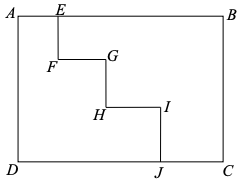
\includegraphics[width=0.4\textwidth]{StarGen/AIMO Trial G3-4 2024/octagon.png}
    \end{figure}
\end{enumerate}

\end{document}